
\documentclass[12pt]{article}
\pagestyle{empty}
\setlength{\parskip}{0in}
\setlength{\textwidth}{6.8in}
\setlength{\topmargin}{-.5in}
\setlength{\textheight}{9.3in}
\setlength{\parindent}{0in}
\setlength{\oddsidemargin}{-.7cm}
\setlength{\evensidemargin}{-.7cm}

\usepackage{amsmath}
\usepackage{amsthm}
\usepackage{amstext}

\usepackage{graphicx}

\begin{document}

{\bf MAT 105 Final Exam (gray) Spring 2009} \hspace{.4in} {\large Name} \hrulefill

\hspace{.2in}

\begin{center}

\begin{tabular}
{|l|c|c|c|c|c|c|c|c|c|c|c|c|c|c|c|c|} \hline

 Problems & \hspace{5 pt} 1 \hspace{5 pt}  & \hspace{5 pt} 2 \hspace{5 pt} & \hspace{5 pt} 3 \hspace{5 pt} & \hspace{5 pt} 4 \hspace{5 pt}& \hspace{5 pt} 5 \hspace{5 pt} & \hspace{5 pt} 6 \hspace{5 pt} & \hspace{5 pt} 7 \hspace{5 pt}   & \hspace{5 pt} 8 \hspace{5 pt} &  \hspace{5 pt} Total  \hspace{5 pt} & &  \hspace{5 pt} Grade \hspace{5 pt}  \\ \hline
&&&&&&&&&&&\\  
Points &&&&&&&&&&   \hspace{.6in}\% &  \\ 
&&&&&&&&&&& \\  \hline
Out of & 40  & 14 & 28 & 22 & 38 & 17 & 22 & 19 &200 & & \\ \hline

\end {tabular}
 
\end{center}

\hspace{.2in}

\begin{itemize}
\item Relax.  You have done problems like these before. Even if these problems look a bit different, just do what you can. 
\item  If you're not sure of something or if you're stuck, please ask! 
\item You may use your calculator but please show all of your work and write down as many steps as you can.  
\item Some formulas from our book that you might need are on a separate sheet.
\item Don't spend too much time on any one problem.
\item  Do well.  And remember to ask me if you need help.
\end{itemize}

  \vspace{.2in}
 
 \hrulefill
 
\newpage  %%%

\begin{enumerate}
\item Evaluate each of the following expressions.

\begin{enumerate}
\item $39.99 + 1.17(200)=$
\vfill
\item $(14)^2-4(-16)(5)=$
\vfill
\item $1,200(1.03)^{72}=$
\vfill
\item $\displaystyle \frac{-(14)}{2(-16)}=$
\vfill
\item $2^{60}=$
\vfill
\item $(5.8)^{1/6}=$
\vfill
\item $\sqrt{354}=$
\vfill
\item $\displaystyle \frac{\text{log}(24.33)}{\text{log}(1.06)}=$
\vfill
\emph{Write the next answer in normal (expanded) decimal notation.}
\item $4.35 \times 10^{6}=$  


\vfill
\emph{Write the next answer in normal (expanded) decimal notation.}
\item $4.35 \times 10^{-6}=$  


\vfill
\end{enumerate}

\newpage  %%%

\item The 1918 flu season was one of the deadliest in history.  The graph and table show the number of flu deaths in London during 1918.

\begin{center}
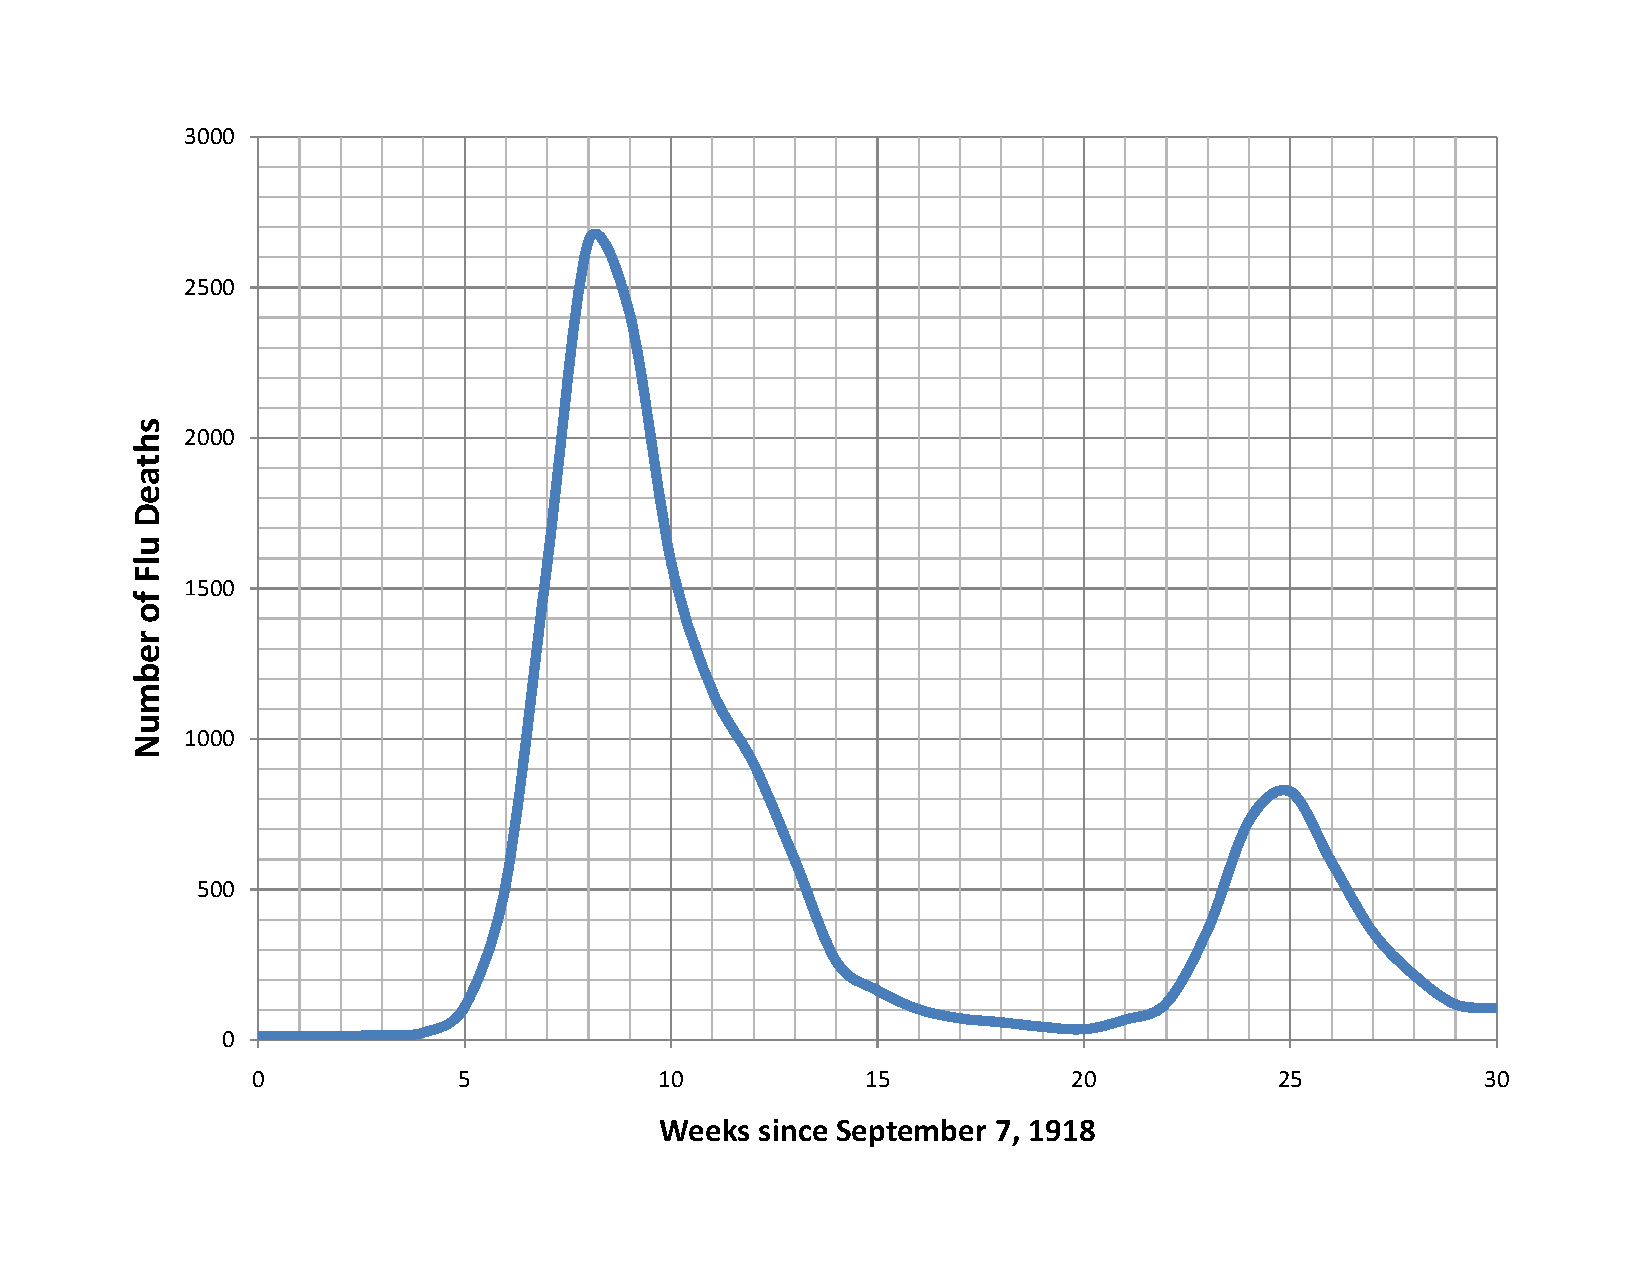
\includegraphics [width = .7\textwidth] {LondonFlu.pdf}
\end{center}

\begin{tabular} {|c|c|c|c|c |c|c|c|c|c |c|c|} \hline
Weeks since Sept. 7, 1918 & 0 & 3 & 6  & 9  & 12  & 15  & 18 & 21  & 24  & 27  & 30 \\ \hline
Number of deaths &13 & 17 & 519 & 2413 & 918 & 165 & 59 & 68 & 729 & 359 & 106 \\ \hline
\end{tabular}

\begin{enumerate}
\item How many people died from the flu 6 weeks after September 7?
\vfill
\item In what week after September 7 did the number of flu deaths drop back to the level at 6 weeks?
\vfill
\item In what week after September 7 was the number of flu deaths the highest and what were the approximate number of deaths?
\vfill
\item Was the number of weekly flu deaths increasing faster 6 weeks after September 7 or 21 weeks after September 7?  Explain.
\vfill
\end{enumerate}

\newpage %%%

\item My plumber charges $P$ dollars for $H$ hours of work, as given by the following formula:
$$P = 57.95 + 95.00H$$

\begin{enumerate}
\item Make a table of values showing the charges for 1 hour, 1$\frac{1}{2}$ hours, 2 hours, and 3 hours.
\vfill
\item What does the 57.95 represent and what are its units?
\vfill
\item What does the 95.00 represent and what are its units?
\vfill
\item If the bill for my plumber's last visit was $\$604.20$, how much time did she work?

\emph{Set up and solve an equation to answer the question.  If you can't solve it, then you may estimate the answer to two decimal places for possible partial credit.}
\vfill
\vfill
\vfill
\item Convert your answer to the nearest minute.
\vfill
She worked for \hrulefill hours, \hrulefill minutes. \hspace{3in}.
\end{enumerate}

\newpage %%%
%% http://aa.usno.navy.mil/data/docs/RS_OneYear.php
\item The timing of the sunset depends on the latitude (how far North of South of the equator one is) and the time of year.  In Minneapolis, the sunset occured at 6:01 PM on March 1.  The time of the sunset is expected to occur 1.26 minutes later each day.  In Galveston, Texas, the sunset occured at 6:19 PM on March 1 and is expected to occur 0.58 minutes later each day.  (Note: do not worry about Daylight Savings Time.) If we let $S$ represent the time of the sunset (in minutes since 6 PM) for $D$ days after March 1, then the equations are:

\vspace{.1in}

\begin{center}
\begin{tabular} {ll} 
Minneapolis: &$S=1+1.26D$ \\
Galveston: & $S=19+0.58D$ \\
\end{tabular}
\end{center}

The table shows sunset times for the two cities:

\begin{center}
\begin{tabular} {|l|r|r|r|r|} \hline
$D$ & 0 & 5 & 15 & 31 \\ \hline
$S$ (Minneapolis) & 1 &  7.3 & 19.9 & 40.1  \\ \hline
$S$ (Galveston) & 19 & 21.9 & 27.7 & 37.0 \\ \hline
\end{tabular}
\end{center}

\begin{enumerate}

\item Which city has a later sunset on March 10 (i.e. after 10 days)?  \emph{Justify your answer.}
\vfill

\item Draw a graph illustrating both equations.
\vspace{.1in}
\begin{center}
\scalebox {.8} {
\includegraphics [width = 6in] {../GraphPaper}}
\end{center}
\vfill
\emph{The problem continues on the next page ...}
\pagebreak
\item Set up and solve an equation to find when the two cities will have the sunset at the same time. Report your answer to the nearest day.

\emph{Just approximating the answer will get almost no partial credit.}

\vfill
\vfill
\vfill
\end{enumerate}

\newpage %%%

\item A diver jumps up in the air from a 3-meter board.  Her height above the water, $H$ meters, after $T$ seconds is given by the formula: $$H = 3 + 5.8T - 4.88T^2$$

\begin{enumerate}
\item Complete the following table of values.

\emph{Please report your answers to two decimal places.}

\begin{center}
\begin{tabular} {|l|c|c|c|c|c|c|} \hline
$T$ & 0 & 0.3 & 0.5 & 0.8 & 1.0 & 1.4 \\ \hline
&&&&&& \\
$H$ & \hspace{.7in} & \hspace{.7in}  & \hspace{.7in}  & \hspace{.7in}  & \hspace{.7in}  & \hspace{.7in}  \\
&&&&&& \\ \hline
\end{tabular}
\end{center}

\item How high up in the air does the diver get?

\emph{Find the answer to two decimal places using whatever method you prefer.}
\vfill
\vfill

\item Convert your answer to the nearest foot.  \emph{Use 1 meter = 3.28 feet.}
\vfill

\hspace{-.5in} \emph{The problem continues on the next page.}

\newpage %%%

\item Draw a graph illustrating the dependence.

\vspace{.1in}
\begin{center}
\scalebox {.8} {
\includegraphics [width = 6in] {../GraphPaper}}
\end{center}
\vspace{.1in}

\item When does the diver hit the water?

\emph{Find the answer to two decimal places using whatever method you prefer.}

\vfill
\end{enumerate}

\newpage %%%
%%% http://www.energywatchgroup.org/fileadmin/global/pdf/2009-01_Wind_Power_Report.pdf

\item Recent reports indicated that the use of windpower to generate energy is growing exponentially.  In 1998, windpower generated 10,000 Mega-Watts of energy.  From 1998 to 2007 energy produced by windpower grew at a rate of 30.4\% per year.  That is, the energy $E$ (in Mega-Watts) produced by windpower $Y$ years after 1998 is given by the equation:

$$E=10000(1.304)^Y$$

\begin{enumerate}
\item According to this equation, how much energy will be produced from windpower in 2009?
\vfill
\item If the value continues to increase, in what year will windpower generate over 200,000 Mega-Watts of Energy?

\emph{Set up and solve an equation to answer the question.  If you can't solve it, then you may estimate the answer for possible partial credit.}
\vfill
\vfill
\vfill
\end{enumerate}

\newpage %%%

\item At Home Depot this week I bought too much stuff to fit in my car, so I rented their truck to haul the stuff to my house.  The table below lists the rental charges for their truck.  Home Depot charges an initial fee plus an hourly rate.

\begin{center}
\begin{tabular} {|r|r|r|r|r|r|r|} \hline
Hours & 1 & 2 & 3 & 4 & 5 & 10 \\ \hline
Cost & \$28.95 & \$38.90 & \$48.85 & \$58.80 & \$68.75 & \$118.50 \\ \hline
\end{tabular}
\end{center}

\begin{enumerate}
\item Name the variables including units.
\vfill
\item What does Home Depot charge per hour to use the truck?
\vfill
\item What is the initial fee?
\vfill
\item Write an equation describing the cost of renting a truck.
\vfill
\end{enumerate}

\newpage %%%

\item My coffee was scalding hot - too hot to drink!  I measured the temperature and found it to be 150 degrees Fahrenheit.  The coffee had cooled to 80 degrees 20 minutes later.  You can assume that the coffee cools exponentially.

\begin{enumerate}
\item By what percentage does the coffee temperature decrease each minute?
\vfill
\item What will the coffee temperature be 10 minutes later (i.e.\ after 30 minutes total)?
\vfill
\end{enumerate}



\end{enumerate}

\end{document}

